%! Author = Sujal Singh
%! Date = 12/3/23

% Preamble
\documentclass[11pt]{beamer}
\title[Derivation for mass-energy equivalence] {Derivation for mass-energy equivalence $[E = mc^2]$}
\author[Chitransh, Divyanshi, Prashant...]
{\(|\) Chitransh Koshta \(|\) Divyanshi Panchal \(|\) Prashant Pulkit \(|\)\\\(|\) Priyanshu Raj
    \(|\) Sujal Singh \(|\)}
\date[Priyanshu, Sujal]{}

\usetheme{Madrid}
\usecolortheme{beaver}
\setbeamertemplate{navigation symbols}{}
\setbeamertemplate{frametitle continuation}[from second][]

% Packages
\usepackage{amsmath}
\usepackage{cancel}
\usepackage{tikz}

\usetikzlibrary{arrows.meta,arrows}

% Document
\begin{document}
    \begin{frame}{Physics Presentation (Group 9)}
        \begin{center}
            %! suppress = FileNotFound
            
\includegraphics[width=80pt]{logo}
        \end{center}\vspace*{-20pt}
        \maketitle
    \end{frame}

    \begin{frame}[t]{Introduction}
        \begin{minipage}[t]{0.65\textwidth}
            In 1905, Albert Einstein published a paper titled \textit{``On the Electrodynamics of Moving Bodies''},
            in which he described the \textbf{Special Theory of Relativity}.\ Using this theory, he derived an equation
            showing mass-energy equivalence:
            \begin{align*}
                E = mc^2
            \end{align*}
            This implied that mass and energy are one and the same and are interchangeable.\\[10pt]
            Let us derive this equation.
        \end{minipage}
        \begin{minipage}[t]{0.05\textwidth}
            ~
        \end{minipage}
        \begin{minipage}[t]{0.1\textwidth}
            \begin{center}
                \vspace*{-10pt}
                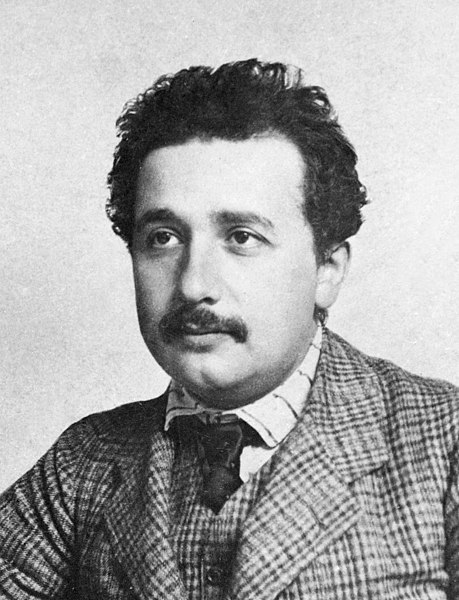
\includegraphics[width=100pt]{albert}
            \end{center}
        \end{minipage}
    \end{frame}

    \begin{frame}[t,allowframebreaks]{Derivation}
        Let us take a particle with resting mass $m_0$, applying force $\vec{F}$ on the particle displaces it by $dx$
        with velocity $\vec{v}$.\\[20pt]

        \begin{minipage}[l]{0.45\textwidth}
            \begin{center}
                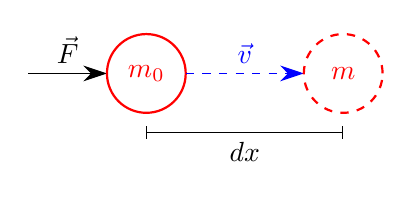
\begin{tikzpicture}
                    \draw [-{Stealth[length=3mm,width=2mm]}] (0,0) -- node[midway,anchor=south] {$\vec{F}$} (1,0);
                    \draw [thick,red] (1.5,0) circle[radius=0.5] node {$m_0$};
                    \draw [-{Stealth[length=3mm,width=2mm]},dashed,blue] (2,0) -- node[midway,anchor=south] {$\vec{v}$} (
                    3.5,0);
                    \draw [thick,red,dashed] (4,0) circle[radius=0.5] node {$m$};
                    \draw [|-|] (1.5,-0.75) -- node[midway,anchor=north] {$dx$} (4,-0.75);
                \end{tikzpicture}
            \end{center}
        \end{minipage}
        \begin{minipage}[r]{0.49\textwidth}
            Calculating the work done,
            \begin{align*}
                dW &= \vec{F}\cdot{d\vec{x}}\\
                &= \left( \frac{d\vec{p}}{dt} \right)\cdot{d\vec{x}}\\
                &= v\cdot{d\vec{p}}\\
                &= v\cdot{d\left( m\vec{v} \right)}\\
                &= v\cdot{\left[ (mdv) + (vdm) \right]}\\
            \end{align*}\vspace*{-40pt}
            \begin{align}
                \boxed{dW = mvdv + v^2{dm}}
            \end{align}
        \end{minipage}

        \framebreak

        To find $mvdv$ using the equation for relativistic mass as derived in previous presentations:\vspace*{-10pt}
        \begin{align*}
            m &= \frac{m_0}{\sqrt{1 - \frac{v^2}{c^2}}}
        \end{align*}~\\\vspace*{-10pt}
        Squaring both sides,\vspace*{-10pt}
        \begin{align*}
            m^2 = \frac{m_0^2 \cdot c^2}{c^2 - v^2}
        \end{align*}\vspace*{-20pt}
        \begin{align}
            \boxed{m^2 c^2 - m^2 v^2 = m_0^2 c^2}
        \end{align}
        Differentiating equation (2):
        \begin{align*}
            c^2 2mdm - (m^2 vdv + v^2 dm) &= 0\\
        \end{align*}~\\\vspace*{-40pt}
        \begin{flushright}[Both $c$ and $m_0$ are constants]\end{flushright}

        \framebreak

        Dividing both sides by $2m$, we get:
        \begin{align*}
            c^2 dm - mvdv - v^2 dm &= 0\\
            \boxed{mvdv = c^2 dm - v^2 dm}
        \end{align*}~\\[-15pt]
        Substituting this value in equation (1):
        \begin{align*}
            dW &= (c^2 dm - \bcancel{v^2 dm}) + \bcancel{v^2 dm}\\
        \end{align*}~\\[-50pt]
        \begin{align}
            \boxed{dW = c^2 dm}
        \end{align}
        Assuming the initial kinetic energy of the particle is 0, let the kinetic energy after applying the force be
        $K$.\ Applying Work-Energy Theorem, we get:
        \begin{align*}
            dW &= dK\\
        \end{align*}

        \framebreak

        Integrating equation (3) and applying limits:
        \begin{align*}
            \int_{0}^{K} dK &= \int_{m_0}^{m} c^2 dm\\[5pt]
            [K - 0] &= c^2 [m - m_0]\\
        \end{align*}~\\[-50pt]
        \begin{align}
            \boxed{K = (m - m_0) c^2}
        \end{align}
        Equation (4) gives the relation for relativistic kinetic energy.
        \begin{align*}
            K &= mc^2 - m_0 c^2
        \end{align*}
        Here, rest mass energy is $m_0 c^2$, which is also the potential energy of the particle.

        \framebreak

        We know,\\[-20pt]
        \begin{align*}
            \text{Total Energy} &= \text{Kinetic Energy} + \text{Potential Energy}\\
            E & = (mc^2 - \bcancel{m_0 c^2}) + \bcancel{m_0 c^2}\\
        \end{align*}~\\[-40pt]
        \begin{align*}
            \LARGE\boxed{E = mc^2}
        \end{align*}
        Hence proved.
    \end{frame}
\end{document}